\section{Задание №8}

Применить метод Монте--Карло к решению первой краевой задачи для двумерного уравнения Лапласа в единичном круге:
$$
        \left\{
\begin{array}{lcr}
        \Delta u=0, \, (x,y)\in D,
\\
        u|_{\delta D}=f(x,y),
\\
        u\in C^2(D), \, f \in C(\delta D),
\\
        D = \{\, x,y \,:\, x^2+y^2 \leqslant 1 \,\}.
\end{array}
        \right.
$$

Для функции $f(x,y)=x^2-y^2$ найти аналитическое решение и сравнить с полученным по методу Монте--Карло.

\subsection{Алгоритм решения задачи}

Построим разностную схему для данной задачи Дирихле. Для этого выберем достаточно мелкую квадратную сетку с шагом~$h$. Координаты узлов пусть будут $x_i = ih$, $y_j = jh$, а значения $u(x_i, y_j)$ и $f(x_i,y_j)$ для краткости обозначим за $u_{i,j}$ и $f_{i,j}$.

\begin{definition}
        Будем называть узел сетки~$(i, j)$ \textit{внутренним}, если он и все четыре соседних с ним узла: $(i-1, j), \ (i + 1, j), \ (i, j - 1), \ (i, j + 1)$ принадлежат области~$D + \delta D$; в противном случае узел $(i, j)$, принадлежащий $D + \delta D$, будем называть \textit{граничным}.

        Обозначим за $D_h$ множество всех внутренних точек, а за $\delta D_h$~--- множество всех граничных точек.
\end{definition}

\begin{figure}[h]\label{img:81}
        \noindent
        \centering
        {
                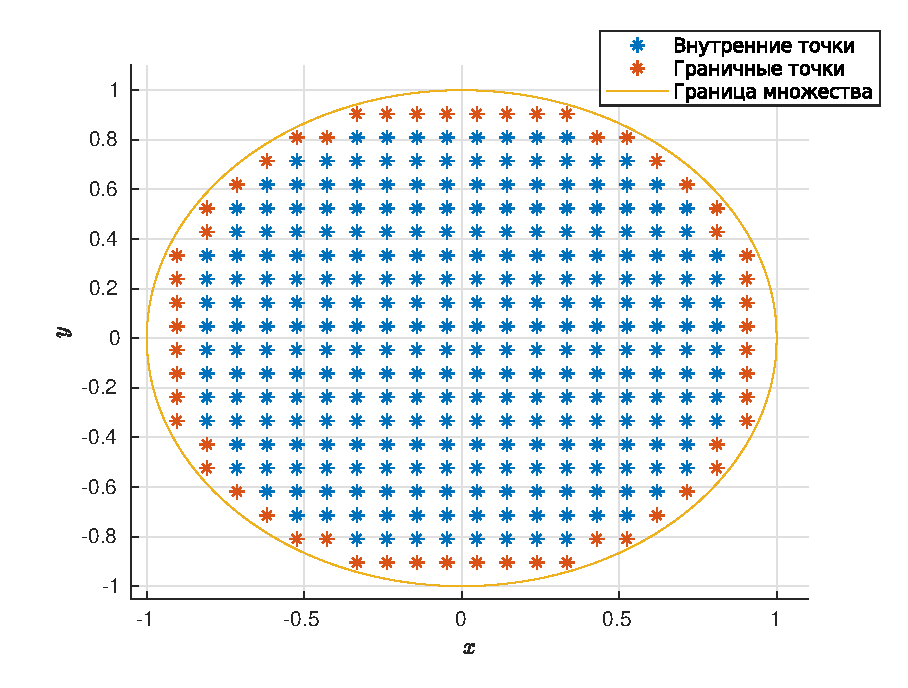
\includegraphics[width=120mm]{task_08/circle.eps}
        }
        \caption{Иллюстрация определения внутренних и граничных точек.}
\end{figure}

Во внутреннем узле $(x_i,y_j)$ уравнение Лапласа $u_{xx}+u_{yy} = 0$ заменим разностным уравнением
$$
\dfrac{u_{i+1,j}-2u_{i,j}+u_{i-1,j}}{h^2} + \dfrac{u_{i,j+1}-2u_{i,j}+u_{i,j-1}}{h^2} = 0,
$$
которое можно переписать в виде
$$
u_{i,j}=\dfrac{1}{4}(u_{i-1,j}+u_{i+1,j}+u_{i,j-1}+u_{i,j+1}).
$$
В граничном же узле положим
$$
u_{i,j}=f_{i,j}.
$$

Представим себе частицу, которая совершает равномерное случайное блуждание по узлам сетки. А именно, находясь во внутреннем узле~$(x_i,y_j)$  сетки, эта частица за один переход с одинаковой вероятностью \nicefrac{1}{4} может переместиться в один из четырёх соседних узлов, причём каждый такой единичный переход случаен и не зависит от положения частицы и истории её передвижений. Будем считать, что блуждание заканчивается, как только частица попадает в граничный узел.

Пусть $P(i,j,p,q)$~--- вероятность того, что траектория частицы, вышедшей из узла~$(x_i,y_j)$, закончится в граничном узле $(x_p,y_q)$. Так как блуждение точки неизбежно заканчивается на границе в первой же точке выхода её на границу, то
$$
        \sum\limits_{(x_p,y_q)\in\delta D_h}P(i,j,p,q)=1,
$$
причём если $(p',q'),\,(p,q) \in \delta D_h$, то
$$
        P(p',q',p,q)
=
        \begin{cases}
1,
        &
\mbox{при $(p'-p)^2+(q'-q)^2=0$,}
        \\
0,
        &
\mbox{при $(p'-p)^2+(q'-q)^2\ne0$.}
        \end{cases}
$$

Теперь составим сумму
$$
        v_{i,j}
=
        \sum\limits_{(x_p,y_q)\in\delta D_h}P(i,j,p,q)f_{pq}.
$$
Если рассматривать функцию~$f(x,y)$ как случайную величину, принимающую значения~$f_{pq}$ на границе~$\delta D_h$, то написанная выше сумма представляет собой математическое ожидание функции~$f(x,y)$ на границе~$\delta D_h$ для траекторий, начинающихся в узле~$(x_i,y_j)$. Тогда в силу закона больших чисел можно аппроксимировать математическое ожидание выборочным средним:
$$
        v_{i,j}
\approx
        \frac{1}{N}\sum\limits_{k=1}^{N}f\left(x_p^{(k)},y_q^{(k)}\right).
$$
Частица, начавшая своё случайное блуждание из внутреннего узла~$(x_i,y_j)$, после первого шага с вероятностью, равной \nicefrac{1}{4}, попадает в один из соседних четырёх узлов. Откуда по формуле полной вероятности
\begin{multline*}
        v_{i,j}
=
        \frac{1}{4}\sum\limits_{(x_p,y_q)\in\delta D_h}(P(i-1,j,p,q)+P(i+1,j,p,q)+P(i,j-1,p,q)+P(i,j+2,p,q))f_{pq}
=\\=
        \frac{1}{4}(v_{i-1,j}+v_{i+1,j}+v_{i,j-1}+v_{i,j+1}).
\end{multline*}
То есть во внутреннем узле~$(x_i,y_j)$

$$
v_{i,j}=\frac{1}{4}(v_{i-1,j}+v_{i+1,j}+v_{i,j-1}+v_{i,j+1}),
$$
а в границном узле
$$
v_{i,j}=f_{i,j}.
$$

Теперь мы можем описать алгоритм построения численного решения задачи:

\begin{enumerate}
        \item Построим квадратную сетку с шагом~$h$ на заданном множестве~$D$, как это сделано, например, на рисунке~8.1.
        \item В каждом граничном узле этой сетки положим
$$
        u(x,y) = f(x,y).
$$ 
        \item В каждом же внутреннем узле~$(x_i,y_j)$ сетки проведем $n$ случайных блужданий. Тогда значение искомой функции в этом узле можно положить
$$
        u(x_i, y_j) = \frac{1}{n} \sum_{k=1}^{n} f(x_{k_i}, y_{k_j}), 
$$
        где $(x_{k_i}, y_{k_j})$~--- граничный узел, в котором завершилось $k$-ое случайное блуждание, ``выпущенное'' из узла $(x_i,y_j)$.
\end{enumerate}


Проверим правильность работы приведенного алгоритма для конкретной функции
$f(x,y) = x^2 - y^2$.
Для того, чтобы нам было с чем сравнивать, найдем аналитическое решение этой задачи.
Сразу оговоримся, что по теореме о существовании решения внутренней задачи Дирихле, оно точно существует.
Будем искать решение в виде
$u(x,y)=Ax^2+By^2+C$.
Подставив его в формулировку задачи, получим следующие условия на коэффициенты:
\[
\left\lbrace
\begin{array}{rcl}
A+B&=&\;\;\,0,\\
A-B&=&\;\;\,2,\\
B+C&=&-1;
\end{array}
\right.\quad\Longleftrightarrow\quad
\left\lbrace
\begin{array}{rcl}
A&=&\;\;\,1,\\
B&=&-1,\\
C&=&\;\;\,0;
\end{array}
\right.
\]

То есть мы получили, что функция
$u(x,y)=x^2-y^2$
является решением задачи, и причём это решение единственно.

\clearpage

\begin{figure}[t]
        \noindent
        \centering
        {
                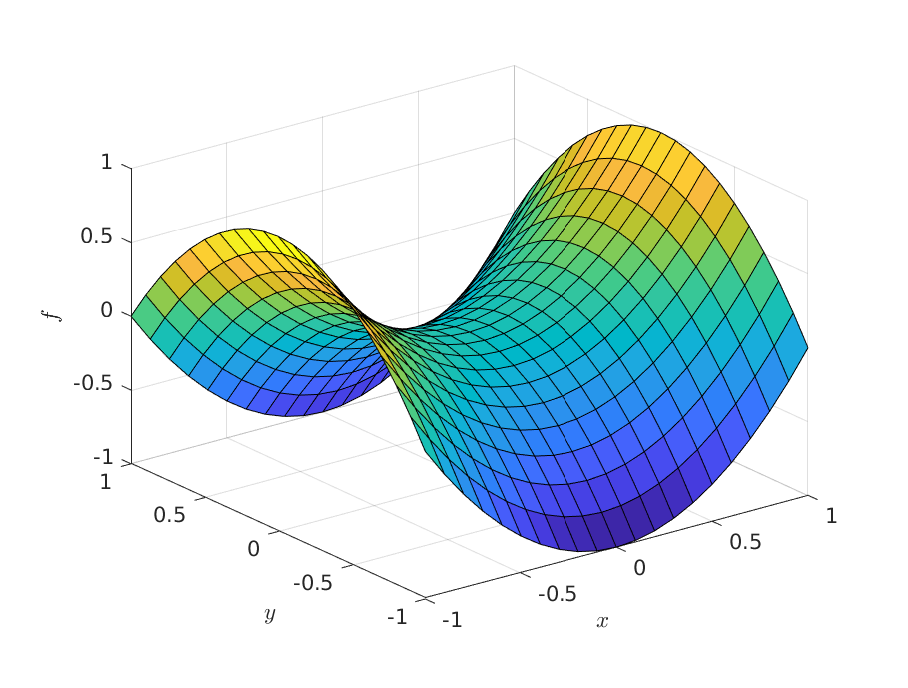
\includegraphics[width=120mm]{task_08/anal.eps}
        }
        \caption{Аналитическое решение задачи, построенное на множестве $[-1,1]\times[-1,1]$.}
\end{figure}
\begin{figure}[b]
        \noindent
        \centering
        {
                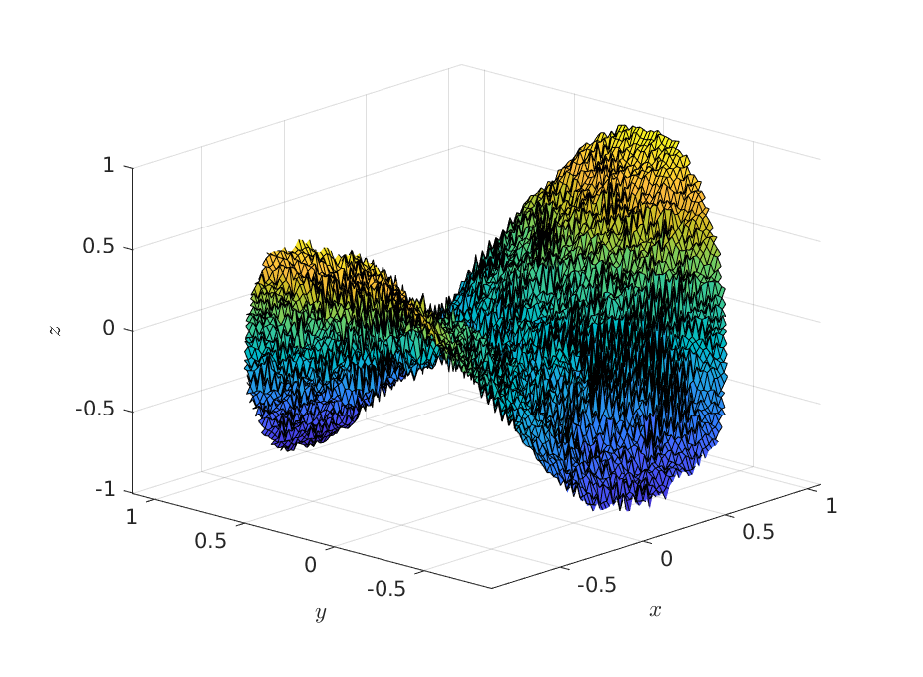
\includegraphics[width=120mm]{task_08/prac.eps}
        }
        \caption{Решение задачи методом Монте--Карло на сетке с радиусом $0,\!02$.}
\end{figure}